\documentclass[technicalreport]{ieicej}
%\documentclass[technicalreport,usejistfm]{ieicej}
\usepackage[dvipdfmx]{graphicx}
\usepackage{latexsym}
%\usepackage[fleqn]{amsmath}
\usepackage{amsmath}
\usepackage{amssymb}
\usepackage{multirow,eepic}
\usepackage{cite}
\usepackage{mediabb}
\usepackage{url}
\usepackage{subfigure}
\usepackage{comment}
\usepackage{epsfig}
\setlength{\oddsidemargin}{-9mm}
\setlength{\evensidemargin}{-9mm}
\setlength{\topmargin}{-4mm}
%\renewcommand{\topfraction}{1.0}
%\renewcommand{\bottomfraction}{1.0}
%\renewcommand{\dbltopfraction}{1.0}
%\renewcommand{\textfraction}{0.01}
%\renewcommand{\floatpagefraction}{1.0}
%\renewcommand{\dblfloatpagefraction}{1.0}
\setcounter{topnumber}{5}
\setcounter{bottomnumber}{5}
\setcounter{totalnumber}{10}

\newcommand{\sij}{(i,\ j)}
\newcommand{\mN}{{\mathcal N}}
\newcommand{\pij}{p^{(i,\ j)}}
\newcommand{\rd}{r^{\sij}_{\rm d}}
\newcommand{\ru}{r^{\sij}_{\rm u}}
\newcommand{\rij}{r^{\sij}}

\jtitle{QoS向上に向けた送信機会の最適化}
%\jsubtitle{}
\etitle{Transmission Opportunity Optimization for QoS improvement}
%\esubtitle{}
 \alignorder=4
 \breakauthorline{4}

\authorlist{%
 \authorentry[info16@imc.cce.i.kyoto-u.ac.jp]{飯田 直人}{Naoto Iida}{^1}
 \authorentry{西尾 理志}{Takayuki NISHIO}{^1}
 \authorentry{守倉 正博}{Masahiro MORIKURA}{^1}
 \authorentry{山本 高至}{Koji YAMAMOTO}{^1}
 \authorentry{鍋谷 寿久}{Toshihisa Nabetani}{^2}
 \authorentry{青木 亜秀}{Tsuguhide Aoki}{^2}
 }

\affiliate[^1]{京都大学 大学院情報学研究科\hskip1zw
  〒606-8501 京都市左京区吉田本町}
 {Graduate School of Informatics, Kyoto University\hskip1em
  Yoshida-honmachi, Sakyo-ku, Kyoto,
  606-8501 Japan}
\affiliate[^2]{株式会社東芝 研究開発センター\hskip 1zw 〒212-8582 神奈川県川崎市幸区小向東芝町1}
  {Corporate Research \& Development Center, TOSHIBA Corporation\hskip1em
   1 Komukaitoshiba-cho, Saiwai-ku, Kawasaki-shi, Kanagawa 212-8582, Japan}

\begin{document}
\begin{jabstract}
	全二重通信無線LANでは送信と受信を同時に同じ周波数帯で行うため,一方向全二重通信の場合,
	所望信号に自身の送信信号が影響を与える自己干渉と,
	送信信号が別の端末(STA)の受信信号に影響を与える端末間干渉が問題となる.
	既にこれらの干渉を考慮した上で,全二重通信を行う端末(STA)の組み合わせを決定する手法が検討されている.
	しかし,それらの手法では自己干渉や端末間干渉の量に応じて変動する受信成功確率やシステムスループットのみによってSTAの組み合わせが決定されるため,
	各STAのアプリケーションの要求の違いを考慮できていない.
	特に,遅延が小さいことが望ましいアプリケーションを用いているSTAであっても,干渉が大きければ送信機会を得にくくなる.
	本稿ではこの問題解決のために,遅延が小さいことが望ましいアプリケーションを用いているSTAの送信機会を最適化し,QoS(Quality of Service)を向上させる手法を提案する.
	さらに,提案手法によりそれらのSTAの遅延時間を削減できることを計算機シミュレーションを用いて示す.
\end{jabstract}
\begin{jkeyword}
全二重通信無線LAN,端末間干渉,最適化
\end{jkeyword}
\begin{eabstract}
	In in-band full-duplex wireless local area networks (WLAN), self-interference and inter-user interference are occur.
	Some authers have already proposed schemes to select two stations(STA) to reduce these interferences.
	However, since these shcemes select STAs based on only the interferences, they cannot take into account application requests like need short delay time.
	In this paper, we propose transmission opportunity optimization for quality of service (QoS) improvemnt.
	The simulation results show that the proposed method reduces the delay time and improves QoS.
	\newline
	\newline
	\newline
	\newline
	\newline
\end{eabstract}
\begin{ekeyword}
full-duplex wireless LAN, inter-user interference, optimization
\end{ekeyword}

\maketitle

\section{はじめに}\label{sec:intro}
	近年,無線LAN(Local Area Network)が急速に普及し,急増するトラヒックにより2.4\,GHz帯は逼迫しており,
	近い将来5\,GHz帯も同様の状態になることで, スループットの低下が問題となる.
	そのような状況において,無線LANシステムの大容量化が望まれる.
	大容量化を実現する方法の一つとして,送信と受信を同時に同じ周波数帯で行う全二重通信無線LANが有望である.
	全二重通信無線LANでは送信と受信を同時に同じ周波数帯で行うため,理想的には周波数利用効率を2倍にすることができる.
	\par
	しかし,全二重通信無線LANでは図\ref{fig:topology}に示すような従来の半二重通信では存在しなかった二つの干渉が問題となる.
	一つは,送受信を行っているAP(Access Point)において,送信信号が所望の受信信号に干渉を及ぼす自己干渉であり,
	もう一つは,STAの送信信号がもう一方のSTAの受信信号に干渉を及ぼす端末間干渉である.
	自己干渉は自己干渉キャンセル技術によって無視できるレベルまで削減できることが示されている~\cite{fdmac, stanford1}.
	また,端末間干渉に関しても,適切なSTAの組み合わせを選び出したり,
	送信電力制御を行ったりすることで端末間干渉を削減する手法が提案されている~\cite{contra, promac}.
	しかし,~\cite{contra, promac}ではSTAの組み合わせを選び出すために過去の全二重通信の成功確率や推定スループットを用いるため,
	端末間干渉の影響しか考慮しておらず,STA間の公平性や各STAが利用しているアプリーケーションの要求の違いが考慮されていない.
	\par
	筆者らは既に~\cite{promac}の最適化問題を改良する形でSTA間の送信機会の公平性を改善する手法を提案している.
	詳細は\ref{sec:fair}節で述べるが,送信待機時間が長いSTAほど送信機会を得やすくすることによって公平性の改善を行った.
	\par
	本稿では,各STAが利用しているアプリケーションの要求の違い,特に低遅延を要求するSTAが混在している場合において,
	それらのSTAの送信機会を最適化しQoSを改善させる手法を提案する.
	さらに,提案手法の有効性を計算機シミュレーションによって評価する.
	\par
	本稿の構成は以下のとおりである.第2章で本稿で扱うシステムモデルについて述べ,第3章では既存の研究と筆者らの過去の提案について述べる.
	さらに,第4章において提案手法について述べ,第5章では提案手法の有効性をシミュレーションによって評価する.
	最後に第5章でまとめとする.

\section{システムモデル}
	\begin{figure}[t]
		\centering
		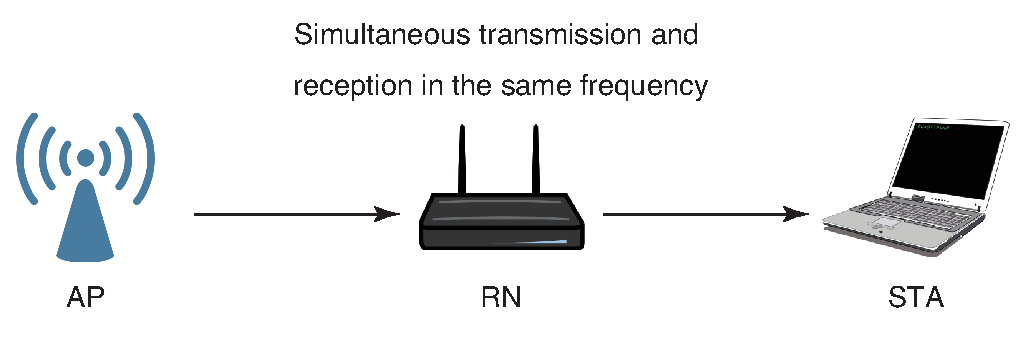
\epsfig{file=fig/model_relay.eps, scale=0.4}
		\label{fig:topology}
	\end{figure}
	\begin{figure}[t]
		\centering
		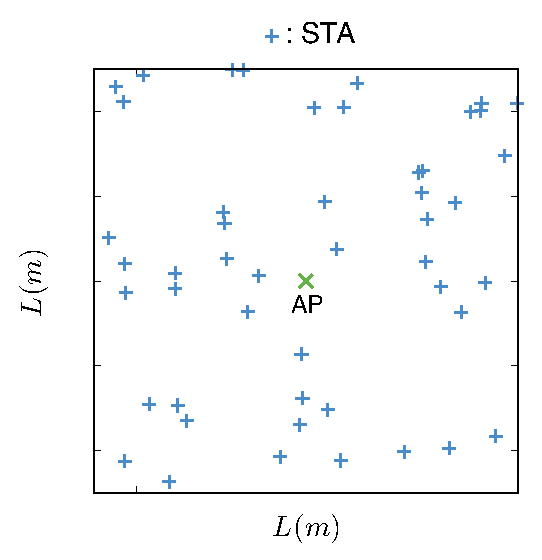
\epsfig{file=fig/pos.eps, scale=0.6}
		\label{fig:model}
	\end{figure}

	本稿で検討するシステムモデルを図\ref{fig:model}に示す.
	1台のAPが$L$四方の領域の中心に設置され,その周りに$N$台のSTAがランダムに配置されているとする.
	それらSTAのインデックス集合を$\mN=\{1,2,...,N\}$とする.
	この$N$台のSTAの中から,図\ref{fig:topology}のようにAPからの下り通信を受信するSTA $i$と,
	APへの上り通信を行うSTA $j$を選び出す.
	このとき,STAの組み合わせを$\sij$と表現し,$i,\ j=\{0\}\cup \mN$であり,$i\neq j$とする.
	ただし,$i=0$のときは上り通信のみの半二重通信,
	$j=0$のときは下り通信のみの半二重通信であるとする.
	さらに,この$N$台のSTAの中に遅延が小さいことが望ましいアプリケーションを用いているSTAが$n$台存在し,
	そのインデックス集合を${\mathcal D}\subset\mN$とする.

\section{関連研究}
	\subsection{Probabilitsic-based adaptive medium access control}
		本節では~\cite{promac}のMACプロトコルについて述べる.
		このMACプロトコルでは,組み合わせ$\sij$で全二重通信が行われる確率$\pij$に基づいてSTA $i$,$j$が決定される.
		\par
		まず,全二重通信の組み合わせ
		\begin{equation}
		{\mathcal C}_{\rm full} \triangleq \{\sij : i,j\in{\mathcal N},\ i\neq j,\ r^{\sij}_d,\ r^{\sij}_u>\epsilon\}
		\end{equation}
		に対して,上り下りそれぞれの実効スループット$\rd$,$\ru$を求め,その合計を$\rij$とする.
		さらに,半二重通信の組み合わせ
		\begin{equation}
			{\mathcal C}_{\rm half} \triangleq \{\sij : i=0\ {\rm or}\ j=0,\ \rij >\epsilon\}
		\end{equation}
		に対しても実行スループット$\rij$を求める.
		得られた$\rij$に基づいて以下の最適化問題を解き,確率$\pij$を得る.
		\begin{align}
			&{\mathcal P}_1: && {\rm max} \sum_{(i,j)\in{\mathcal C}} p^{(i,j)}r^{(i,j)} &&&&&& \label{eq:p1}\\
			&{\rm subject\ to} && \sum_{j\in\{j:(i,j)\in{\mathcal C}\}} p^{(i,j)} \geq \eta_d^{(i)}, \forall i\in {\mathcal N}  \\
			&&& \sum_{i\in\{i:(i,j)\in{\mathcal C}\}} p^{(i,j)} \geq \eta_u^{(j)}, \forall j\in {\mathcal N}  \\
			&&& \sum_{j\in\{j:(i,j)\in{\mathcal C}\}} p^{(i,j)}=1 \\
			&{\rm variables:} &&p^{(i,j)} \in {\mathbb R}_{\geq 0},\forall(i,j)\in {\mathcal C}
		\end{align}
		ただし,${\mathcal C} = {\mathcal C}_{\rm full} \cup {\mathcal C}_{\rm half}$であり,
		$\eta_d^{(i)}$はSTA $i$への下り通信のトラヒックに比例した値,
		$\eta_u^{(j)}$はSTA $j$が持つ上り通信のトラヒックに比例した値である.
		\par
		次に,得られた$\pij$からSTA $i$,$j$を決定する方法を述べる.
		APは
		\begin{equation}
			p_{\rm d}^{(i)}= \sum_{j\in\{j:(i,j)\in{\mathcal C}\}}p^{(i,j)},\forall i \in \{0\}\cup{\mathcal N}
		\end{equation}
		によって各STAが下り通信の送信先となる確率$p_d^{(i)}$を求め,この確率に従ってランダムに送信先を選択する.
		さらに,
		\begin{equation}
			p_{\rm u}^{(j)} = P(j\ {\rm wins\ uplink|AP\ sends\ to}\ i)=\pij / p_{\rm d}^{(i)}
		\end{equation}
		によって得られた条件確率$p_{\rm u}^{(j)}$を用いて$CW^{\sij}_{\rm u}$を
		\begin{equation}
			CW^{\sij}_{\rm u} = \lceil 1/p_{\rm u}^{(j)} \rceil
		\end{equation}
		と求め,$CW^{\sij}_{\rm u}$をコンテンションウィンドウサイズとしたバックオフアルゴリズムによってSTA $j$が決まる.

	\subsection{公平性の改善}\label{sec:fair}
		筆者らは先の研究において,~\cite{promac}の各STAの送信機会の公平性を改善するための検討を行った.
		最初に述べたようにこのMACプロトコルでは干渉が小さい組み合わせが選ばれやすく,
		STA間の公平性が低下するという問題点がある.
		この問題を解決をするため待機時間を考慮にいれることを提案した.
		待機時間とはあるSTAのバッファの先頭にフレームが到着してから送信されるまでの時間である.
		最適化問題の式\eqref{eq:p1}に以下のように待機時間$d^{(j)}$の項を加え,
		\begin{equation}
			{\mathcal P}_2: {\rm max} \sum_{(i,j)\in{\mathcal C}} p^{(i,j)}r^{(i,j)}(d^{(j)})^{\alpha} \label{eq:p2}
		\end{equation}
		とすることで送信機会の公平性が改善できた.一方,公平性が高くなるとシステムスループットが低下することもわかった.
		そのため重み付けの$\alpha$を変化させることで,公平性とシステムスループットのバランスをシステムの要求に応じて変化させられることを示した.

\section{提案方式}
\begin{align}
	&{\mathcal P}_3: && {\rm max} \sum_{(i,j)\in{\mathcal C}} p^{(i,j)}r^{(i,j)}(d^{(j)})^{\alpha} &&&&&&\\
	&{\rm subject\ to} && \sum_{j\in\{j:(i,j)\in{\mathcal C}\}} p^{(i,j)} \geq \eta_d^{(i)}, \forall i\in {\mathcal N}  \\
	&&& \sum_{i\in\{i:(i,j)\in{\mathcal C}\}} p^{(i,j)} \geq \eta_u^{(j)}-x, \forall j\in {\mathcal N}_{\rm {\overline D}}  \\
	&&& \sum_{i\in\{i:(i,j)\in{\mathcal C}\}} p^{(i,j)} \geq \eta_u^{(j)}+y, \forall j\in {\mathcal N}_{\rm D}  \\
	&&& \sum_{j\in\{j:(i,j)\in{\mathcal C}\}} p^{(i,j)}=1 \\
	&{\rm variables:} &&p^{(i,j)} \in {\mathbb R}_{\geq 0},\forall(i,j)\in {\mathcal C}
\end{align}


\section{シミュレーション}


\section{まとめ}

\bibliographystyle{sieicej}
\bibliography{main2}

\end{document}
